% Chapter 1
% !TeX spellcheck = en_US 
\chapter{Statistical Learning Theory} % Main chapter title

\label{Chapter2} % For referencing the chapter elsewhere, use \ref{Chapter1} 
\setcounter{chapter}{2}
%----------------------------------------------------------------------------------------
In the previous chapter we have observed the phenomenon of overfitting; a model
trained to minimize the empirical risk on a training dataset can still fail to generalize
well over unseen dataset. A fundamental question in statistical learning theory is how to design
hypothesis classes that do not overfit.  

We will see in this chapter that restricting the complexity of the hypothesis classes can help
reduce the overfitting. First, we start by looking at finite hypothesis classes
and show that they do not overfit. This result will also motivate a notion of statistical learning, that of \emph{probably approximately correct
(PAC)} learning. However, finiteness of the hypothesis class is, indeed, a very
restricting condition. We will discuss other measures of the complexity of a
hypothesis class, such as the \emph{Vapnik-Chervonenkis (VC) dimension} and the
\emph{Rademacher complexity}. At the end of this chapter, we will discuss what
these theoretical results imply for the design of machine learning algorithms and
link to the concept of \emph{overparameterization}, which is a hot topic in the field of deep learning.

The reader is referred to~\cite{Shalev:ML:2014} and~\cite{Shapire:ThML2019} for more details. 

We start this section by recalling some basic definitions of probability
measure theory.
\section{Probability Measure Theory}
As we have seen in \nameref{Chapter1}, training datasets are treated as random
variables. This makes the following tools from probability theory essential. 

Let $(\Omega,\mathcal{A}, \mathbb{P})$ be a probability measure space, where $\Omega \subseteq \mathbb{R}$. 
It is common to refer to any $A \in \mathcal{A}$ by an \emph{event}. An event
$A$ s.t. $\mathbb{P}(A)=1$ is said to happen \emph{almost surley.}

Important probability measures are those induced by measurable transformations in the following way. 
\begin{definition}[Push-forward Measure]
	Given two measurable spaces $(\Omega_1, \mathcal{A}_1)$, $(\Omega_2, \mathcal{A}_2)$ and a measurable mapping $h:\Omega_1 \to \Omega_2$ 
	the \emph{push-forward measure} of a measure $\mathbb{P}$ on $(\Omega_2, \mathcal{A}_2)$ is 
	$$
	h_\#\mathbb{P} (A) := \mathbb{P} (h^{-1}(A)) \quad  \forall A \in \mathcal{A}_2.
	$$
	The push-forward measure is sometimes denoted by $\mathbb{P} h^{-1}$.
\end{definition}

We look now at a special kind of measurable mappings and the measures they induce.
\begin{definition}[Real Random Variables and Distributions]
	\label{def:RV}
	\begin{enumerate}[(i)] Let $(\Omega,\mathcal{A}, \mathbb{P})$ be a probability measure space.
		\item A measurable mapping $V: \Omega \to \mathbb{R}$ is called a \emph{real random variable}.
		\item The push-forward measure $\mathcal{P}_V := V_\# \mathbb{P}$ induced by a real random variable $V$ 
		is called the \emph{(probability) distribution of $V$}.		
	\end{enumerate}
\end{definition}
A mapping $V: \Omega \to \mathbb{R}^n$ for $n>1$ is usually referred to as a
\emph{random vector}. In our treatment we will refer to $V$ by a random variable
for any $n\geq 1$. 
\begin{definition}[Expected Value]
	\begin{itemize}
		\item The expected value of a random variable $X: \Omega \to
		\mathbb{R}$, denoted by $\mathbb{E}[X]$
		is defined as:
		\begin{align*}
			\mathbb{E}[X] &:= \int_\Omega X(\omega) \ d\mathbb{P}(\omega) \\
			& = \int_\mathbb{R} x \ d\mathcal{P}_X(x),
		\end{align*}
		where $\mathcal{P}_X$ is the pushforward-measure of $X$.
		\item Similarly, the expected value of a measurable mapping $g:
		\mathbb{R}\to \mathbb{R}$ as a function of the random variable $X$ is given by 
		\begin{align*}
			\mathbb{E}[g(X)] &:= \int_\Omega g(X)(\omega) \ d\mathbb{P}(\omega) \\
			& = \int_\mathbb{R} g(x) \ d\mathcal{P}_X(x).
		\end{align*}
		Sometimes, one writes $\mathbb{E}[g] = \mathbb{E}_{x \sim \mathcal{P}_x}[g]$
		to highlight the measure on $\mathbb{R}$ against which one integrates.
	\end{itemize}
\end{definition}


\begin{definition}[Independent Events]
Two events $A,B$ are said to be \emph{independent} if $$\mathbb{P}(A \cap B) = \mathbb{P}(A)\mathbb{P}(B).$$ Given 
an index set $I$, consider the family $A_i \in \mathcal{A}$ for $i \in I$. The
family $(A_i)_{i\in I}$ of events is said to be \emph{independent}
if $$\mathbb{P}(\cap_{j \in J} A_j) = \prod_{j \in J} \mathbb{P}(A_j) \quad \forall J \subset I.$$	
\end{definition}

The independence of events (i.e., sets) can be generalized to independence of
families of sets. 
\begin{definition}[Independence of Families of Sets]
        Let $I$ be an index set and consider $\mathcal{E}_i \subseteq \mathcal{A}$ for all $i \in I$.
        The family $(\mathcal{E}_i)_{i \in I}$ is called \emph{independent} if, for any finite subset 
        $J \in I$ and any choice of $E_j \in \mathcal{E}_j, j \in J$, one has 
        $$
        \mathbb{P}(\cap_{j \in J} E_j) = \prod_{j \in J} \mathbb{P}(E_j).
        $$
\end{definition}
The following is an important family of random variables that one often encounters 
in machine learning and statistics. 
\begin{definition}[Independent and Identically Distributed Random Variables]
	\label{def:iid}
	Let $I$ be an index set and $(V_i)_{i \in I}$ be a family of real random 
	variables. Endow $\mathbb{R}$ with the Borel $\sigma$-algebra $\mathcal{B}$.
	\begin{enumerate}[(i)]
		\item The family $(V_i)_{i \in I}$ is said to be \emph{identically distributed} if 
		$$\mathcal{P}_{V_i} = \mathcal{P}_{V_j} \quad \text{ for all } i, j \in I.$$
		\item The family $(V_i)_{i \in I}$ is said to be \emph{independent} if the 
		family of generated $\sigma$-algebras $\bigl(\sigma(V_i) \bigr)_{i\in I}$, where 
		$\sigma(V_i) = V_i^{-1}(\mathcal{B})$ is independent.
	\end{enumerate}
A family of real random variables satisfying both conditions is said to be
\emph{independent and identically distributed (i.i.d.)}.
In such a case set $\mathcal{P} = \mathcal{P}_{V_i}$. \end{definition}

\section{A Formal Setting of Learning}
\label{sec:formal_learning}
We start by defining the standard setting of supervised learning. In our
treatment, we will not use this very general setting. We will be imposing restrictions, for
example, by considering only binary classification problems, or by using special
loss functions. Nevertheless, it is useful to see the general setting first.

Let $z = (x, y)$ be a random variable where $x: \Omega \to \mathbb{X} \subseteq
\mathbb{R}^n$ and $y: \Omega \to \mathbb{Y} \subset \mathbb{R}$. Denote by
$\mathcal{P}$ the probability distribution of $z$ and by $\mathcal{P}_x$ the
marginal probability distribution corresponding to the random variable $x$.
Further, we set $\mathbb{Z} := \mathbb{X} \times \mathbb{Y}$ \footnote{Do not
confuse the notation with the set of integers.}. We denote by $p(z)$ and $p(x)$
the probability density functions of $z$ and $x$, respectively. These two
densities are related by the formula $p(z) = p(x)p(y|x)$.

Given a hypothesis class $\mathfrak{H}$ of functions $h: \mathbb{X} \to \mathbb{Y}$ and a loss function $l:\mathbb{Y}^2 \to \mathbb{R}_{>0}$, the goal of a supervised-learning
algorithm is to solve 
\begin{equation*}
    \underbrace{R_{\mathcal{P}}(h) := \int_{\mathbb{Z}} l(y, h(x)) \ d \mathcal{P}}_{\text{True risk}} \longrightarrow \min_{h \in \mathfrak{H}} \implies h^\star, 
\end{equation*}
that is, to minimize the \emph{true risk}. Note that the true risk is also called the
\emph{generalization error}. However, one only has access to a finite
realiazation of the random variable $z$, i.e., to a training set $D=\{(x_i,
y_i)_{i=1}^m\}$. A reasonable thing to do is, hence, to minimize a
finite/empirical representation of the true risk, i.e., to solve
\begin{equation*}
    \underbrace{\hat{R}_{\mathcal{P}} (h) := \sum_{(x,y) \in D} \frac{1}{|D|}l(y, h(x)) }_{\text{Empirical risk}} \longrightarrow \min_{h \in \mathfrak{H}} \implies \hat{h}^\star.
\end{equation*}

A learning algorithm that replaces the original task of minimizing the true risk
by the task of minimizing the empirical risk is called an \emph{empirical risk
minimization (ERM) learner} or
is said to be using the \emph{ERM learning rule}. To highlight the dependence of
the empirical risk on the training data, we sometimes write $\hat{R}_{\mathcal{P}}(h;D)$.

One of the main problems of statistical learning theories is to study the
validity of approximating $h^*$ by $\hat{h}^*$. In particular, under what
conditions on the hypothesis class does $\hat{h}^*$ have a small generalization error?
In the next section, we will see that the finiteness of the hypothesis class is
a sufficient condition to this end. Is it necessary though?

\section{Probably Approximately Correct Learning}

We start this section by looking closely at the problem of overfitting and show that
finite classes do not overfit. Our results to this end motivate a notion of
statistical learning that we discuss.

For this section, we will adopt the setting defined in
\autoref{sec:formal_learning} and further assume that $\mathbb{Y} = \{0,1\}$,
i.e., we restrict ourselves to the binary classification case. Moreover, we
assume that $y$
is generated from $x$ by the deterministic functional relation $y=f(x)$, where $f: \mathbb{X}
\to \{0,1\}$. Unless otherwise stated, we will set the loss function to be the 0-1 loss
which
we define as follows.
\begin{equation*}
    l(y, h(x)) :=
    \begin{cases}
         & 1: \ h(x) \neq y \\
        & 0: \ \text{otherwise}.
    \end{cases}	
\end{equation*}
Note that in this case, the true and empirical risks simplify to
$$
R_{\mathcal{P}}(h) = \mathcal{P}_x \bigl(\{x: h(x) \neq y\} \bigr)
$$
$$
\hat{R}_{\mathcal{P}}(h) = \frac{1}{m} | \{x: h(x) \neq y\} |
$$

Moreover, we restrict ourselves to working under the  
 \emph{realizability assumption}, i.e., that
there exists $h^* \in \mathfrak{H}$ s.t. $R_{\mathcal{P}}(h^*) = 0$. Note that
this assumption implies that the empirical risk of the hypothesis obtained by
the ERM rule is zero, i.e., $\hat{R}(\hat{h}^*) = 0$ with probability 1 over the
choice of the training data. In other words, the realizability assumption
implies that the ERM rule provides a hypothesis that is \emph{consistent} on the
training data. To see this, note that $R_\mathcal{P}(h^*)=0$ implies
that $\hat{R}_\mathcal{P}(h^*;D)=0$ with probability 1 over the choice of a
dataset $D$ that is i.i.d. generated by $\mathcal{P}$. In turn, this implies
that $\hat{R}_\mathcal{P}(\hat{h}^*;D)=0$ with probability 1 over the choice of
$D$ since $\hat{R}_\mathcal{P}(\hat{h}^*;D) \leq \hat{R}_\mathcal{P}(h^*;D)$ by
the definition of the ERM rule.

\subsection{Finite Hypothesis Classes do not Overfit}
The goal in this section is to show that we won't encounter an overfitting
problem if the hypothesis class has finitely many elements. We will deal with
the overfitting problem in an approximate manner, i.e., we will say that a
hypothesis $h$ does not overfit if $R_\mathcal{P}(h)\leq \epsilon$ for some
small $\epsilon>0$.

In what follows, given a dataset $D$, we denote by $D|_x$ the input of the
dataset, i.e., $D|_x=\{x_i: i=1,\dots,m\}$. Note that since each $x\in D|_x$ is a
random variable with a distribution $\mathcal{P}_x$, the dataset $D|_x$ has distribution $\mathcal{P}^m_x$ over $\mathbb{X}^m$.

\begin{lemma}
	\label{lem:PAC_fh}
		Under the realizability assumption and
		for accuracy $\epsilon >0$ it holds that 
		$$
		\mathcal{P}^m_x\bigl(\{D|_x: R_\mathcal{P}(\hat{h}^*) > \epsilon\} \bigr) \leq |\mathfrak{H}| e ^{-\epsilon m}.
		$$
	\end{lemma}
	In words; the probability of sampling $m$ training data points and
	obtaining a learner $\hat{h}^*$ by the ERM rule that does not generalize well is
	upperbounded. Note that this upperbound is finite if the cardinality of
	$\frak{H}$ is finite. Also note that 
	$$
	\mathcal{P}^m_x\bigl(\{D|_x: R_\mathcal{P}(\hat{h}^*) > \epsilon\} = \mathbb{P}_{D|_x \sim \mathcal{P}^m_x} \bigl( \{ R_\mathcal{P}(\hat{h}^*) > \epsilon \}\bigr). 
	$$
\begin{proof}
    We start by defining the set $\mathfrak{H}_b$ of bad hypotheses, i.e., the
    set of all hypotheses that lead to a generalization error $> \epsilon$,
    $$
    \mathfrak{H}_b := \{h \in \mathfrak{H} \text{ s.t. } \mathbb{R}_\mathcal{P} (h) > \epsilon\}.
    $$
    Next, we define the set of misleading training data, i.e., the set of all
    training datasets of cardinality $m$, on which there is at least one
    hypothesis that produces zero training error and a generalization error $>
    \epsilon$,
    $$
    M:= \{D|_x: \ |D|_x|=m, \text{ and s.t. there exists }h  \in \mathfrak{H}_b : \ \hat{R}_\mathcal{P}(h;D)=0 \}.
    $$
    Note that the realizability assumption implies that
    $\hat{R}_\mathcal{P}(\hat{h}^*)=0$ as discussed before. This in turn implies
    that $\{D|_x: R_\mathcal{P}(\hat{h}^*) > \epsilon\} \subseteq M$. It thus
    follows that 
	\begin{align*}
		\mathcal{P}^m_x\bigl(\{D|_x: R_\mathcal{P}(\hat{h}^*) > \epsilon\}\bigr) &\leq \mathcal{P}^m_x(M)\\
		&\leq \sum_{h \in \mathfrak{H}_b} \mathcal{P}^m_x\bigl(\{D|_x: \hat{R}_\mathcal{P}(h;D)=0\}\bigr)\\
		&= \sum_{h \in \mathfrak{H}_b} \prod_{i=1}^m \mathcal{P}_x\bigl(\{x: h(x) = y\}\bigr)\\
		&= \sum_{h \in \mathfrak{H}_b} \prod_{i=1}^m (1-R_\mathcal{P}(h)) \quad {\color{mildred} \text{(definition of true risk)}}\\
		&\leq \sum_{h \in \mathfrak{H}_b} (1-\epsilon)^m \quad {\color{mildred} \text{(since } h \in \mathfrak{H}_b)}\\
		&\leq |\mathfrak{H}_b| (1-\epsilon)^m \\
		&\leq |\mathfrak{H}| (1-\epsilon)^m \\
		&\leq |\mathfrak{H}| e^{-\epsilon m}.
	\end{align*}	
\end{proof}
The above lemma shows that the probability of overfitting is exponentially small
with the size of the training data. It also provides us with a way to find the
minimal amount of training data that guarantees a small generalization error.
    \begin{coro}
		\label{Coro:finite_hypo}
		Let $\mathfrak{H}$ be a finite hypothesis class. Let $\delta \in (0,1)$ be a confidence parameter and $\epsilon \in
		(0,1)$ be an accuracy parameter. Let $m$ be an integer that satisfies
		$$
		m \geq \frac{1}{\epsilon} \log(|\mathfrak{H}|/\delta).
		$$ 	
		Under the realizability assumption it holds that 
		$$
		\mathbb{P}_{D|_x \sim \mathcal{P}^m_x} \bigl( \{ R_\mathcal{P}(\hat{h}^*) > \epsilon \}\bigr) \leq \delta.
		$$
		In other words, 
		$$
		R_\mathcal{P}(\hat{h}^*) \leq \epsilon
		$$
		holds with probability of at least $1-\delta$ over the choice of the
		training data $D$.
	\end{coro}
	Note that this result holds for any labeling function $f$ and any
	distribution $\mathcal{P}_x$. 
    \begin{proof}
        Follows straight-forwardly from the previous lemma.
    \end{proof}
The results we proved so far show that finite hypothesis classes do not overfit.
Here, overfitting is defined in an \emph{approximate sense} controlled by parameter
$\epsilon$. The results guarantee that the ERM rule provides a hypothesis
that generalizes well in a \emph{probabilistic sense}. The probability here is
controlled by a parameter $\delta$. This motivates the following definition.

    \begin{definition}
		A hypothesis class $\mathfrak{H}$ is PAC learnable if there exist a
		function $m_\mathfrak{H}: (0,1)^2 \to \mathbb{N}$ and a learning
		algorithm with the following properties
		\begin{itemize}
			\item for every $(\epsilon, \delta) \in (0,1)^2$
			\item for every distribution $\mathcal{P}_x$ over $\mathbb{X}$
			\item for every labeling function $f: \mathbb{X} \to \{0,1\}$
		\end{itemize}
		s.t. if the realizability assumption holds, when running the learning
		algorithm on $m \geq m_\mathfrak{H}(\delta, \epsilon)$ i.i.d. samples
		generated by $\mathcal{P}_x$ and labeled by $f$, the algorithm returns a
		hypothesis $h$ such that 
		$$
		R_\mathcal{P}(h) \leq \epsilon
		$$ 
		with probability of at least $1-\delta$ over the choice of the samples.
	\end{definition}

    \begin{definition}[samples complexity]
		The sample complexity of leaning a hypothesis class $\mathfrak{H}$ is
		the minimal integer that satisfies the requirement of PAC learnability
		with accuracy $\epsilon$ and confidence $\delta$.
	\end{definition}
	With these definitions we can restate our corollary in the following manner.
	\begin{coro}
		Every finite hypothesis calss is PAC learnable with sample complexity 
		$$
		m \leq \lceil \frac{1}{\epsilon} \log(|\mathfrak{H}|/\delta) \rceil
		$$
	\end{coro}
One may wonder whether the finiteness of the hypothesis class is a necessary
condition for PAC learnability. We will see now that this is indeed not the
case. For example, we consider here the class of threshold functions. 
\begin{definition}[Class of Threshold Functions]
	$\mathfrak{H} := \{h_a:\mathbb{R}\to \{0,1\}, h_a(x)= \mathbf{1}_{x <a} ,\  a\in \mathbb{R}\}$
\end{definition}	
In words, this class consists of all functions that assign 1 to all inputs that
are smaller than a threshold $a$ and 0 otherwise. The class of threshold
functions has infinite cardinality. However, we will see that this class is PAC learnable.
\begin{lemma}
The class of threshold functions	$\mathfrak{H}$ is PAC-learnable using the ERM rule with sample complexity of
	$m_\frak{H} \leq \lceil \frac{1}{\epsilon}\log (2/\delta)\rceil$.
\end{lemma}
\begin{proof}
	It suffices to show that 
	$$
	\mathbb{P}_{D|_x \sim \mathcal{P}^m_x} \bigl( \{ R_\mathcal{P}(\hat{h}^*) > \epsilon \}\bigr) \leq 2 \exp(-\epsilon m).
	$$
	To prove this note that we work under the realizability assumption. Hence,
	it is possible to find a hypothesis $\hat{h}^* = h_{\hat{a}^*}$ that is
	consistent with the training data. 
	
	Let $a^*$ be the threshold of the labeling function $f$. Let $a^* _r >a^*$ be such that $\mathbb{P}_{x \sim \mathcal{P}_x}\bigl(x \in (a^*,
	\hat{a}^*_r)\bigr)= \epsilon$. Similarly, let $a^*_l <a^*$ be such
	that $\mathbb{P}_{x \sim \mathcal{P}_x}\bigl(x \in (\hat{a}^*_l, a^*)\bigr)=
	\epsilon$. Notice that picking datapoints that are outside the interval
	$(a^*_l, a^*)$ or outside $(a^*, a^*_r)$ is a sufficient condition for picking training datasets that lead to a bad
	hypothesis. Formally
	\begin{align*} 
	\mathbb{P}_{D|_x \sim \mathcal{P}^m_x} \bigl( \{ R_\mathcal{P}(\hat{h}^*) > \epsilon \}\bigr) &\leq \mathbb{P}_{D|_x \sim \mathcal{P}^m_x} \bigl(\{\forall x \in D|_x,  x \notin (a^*_l, a^*) \vee x \notin (a^*, a^*_r)\}\bigr) \\
	&\leq \underbrace{\mathbb{P}_{D|_x \sim \mathcal{P}^m_x} \bigl(\{\forall x \in D|_x,  x \notin (a^*_l, a^*) \}\bigr)}_{\text{term} 1} + \mathbb{P}_{D|_x \sim \mathcal{P}^m_x} \bigl(\{\forall x \in D|_x,  x \notin (a^*, a^*_r)\}\bigr). 
	\end{align*}
	Note that 
	\begin{align*}
		\text{term }1 &\leq \mathbb{P}_{D|_x \sim \mathcal{P}^m_x} \bigl(\{x_1 \notin (a^*_l, a^*) \wedge x_2 \notin (a^*_l, a^*) \wedge \dots \wedge x_m \notin (a^*_l, a^*) \}\bigr)\\
		&= \prod_{i=1}^m \mathbb{P}_{x \sim \mathcal{P}_x} \bigl(x \notin (a^*_l, a^*)\bigr)\\
		&= (1-\epsilon)^m.
	\end{align*}
	The claim follows by doing the same inequality for the second term and using $(1-\epsilon)^m \leq \exp(-\epsilon m)$.
\end{proof}
In summary, our results show that finiteness of the hypothesis class is not a
good condition for characterizing PAC learnability, since infinite classes can
be PAC learnable. We thus move in the next section to introduce a better measure
of the complexity of a hypothesis class.

\subsection{Vapnik-Chervonenkis Dimension}
The Vapnik-Chervonenkis (VC) dimension is a measure of the complexity of a
hypothesis class. The intuition behind this measure is to define the richness of
a class with respect to a given dataset. For example, a class of threshold
functions is infinite dimensional. However, given a dataset $D$ of only one
point $x \in \mathbb{R}$, the whole class of threshold functions can give this
datapoint only two
different values, either 0 if the hypothesis has a threshold lying to the
left of the datapoint, or 1 otherwise. Now consider a dataset
of two points. The class of threshold functions can label these two points in three
different ways, (0,0), (1,0) or (1,1). However, the hypothesis class of threshold
functions cannot represent the labeling (0,1). Hence, the class of threshold
functions cannot exhaust all the possible labeling of a dataset of two
points. This is indeed the motivation behind the following definitions.

\begin{definition}[Restriction of $\mathfrak{H}$ to $C$]
	Let $\frak{H}$ be a class of functions from $\mathbb{X}$ to $\{0,1\}$
	and let $C = \{x_1, \dots, x_m\} \subset \mathbb{X}$. The restriction of
	$\mathfrak{H}$
	to $C$ is the set of functions from $C$ to $\{0,1\}$ that can be derived from
	$\mathfrak{H}$. That is, 
	$$
	\mathfrak{H}_C := \{(h(x_1), \dots, h(x_m)): h \in \mathfrak{H}\}.
	$$	
	 \end{definition}
	 If $\mathfrak{H}_C$ is the set of all functions from $C$ to $\{0,1\}$
	 we say that $\mathfrak{H}$ shatters $C$. Formally we write as follows.
	 \begin{definition}[Shattering]
		A hypothesis class $\mathfrak{H}$ shatters a finite set $C \subset
		\mathbb{X}$
		if $|\mathfrak{H}_C|= 2^{|C|}$.
	 \end{definition}
	 According to this definition we observe that the class of threshold
	 functions shatters a set of one point but does not shatter a set of two
	 points, because it does not exhaust all of its possible labelings.

	 The following definition quantifies the number of different labelings that a
	 hypothesis class can provide for a dataset of fixed size.
	 \begin{definition}[Growth Function]
		Let $\mathfrak{H}$ be a hypothesis class. The growth function of
		$\mathfrak{H}$, denoted by $\tau_\mathfrak{H} :\mathbb{N} \to \mathbb{N}$ is defined as 
		$$
		\tau_\mathfrak{H}(m) := \max_{C \subset \mathbb{X}: |C|=m}|\mathfrak{H}_c|
		$$
	\end{definition} 
	In words; $\tau_\mathfrak{H}(m)$ is the maximum number of different functions
	from a set $C$ of size $m$ to $\{0,1\}$ that can be obtained
	by restricting $\mathfrak{H}$ to $C$.

	It turns out that the growth function is a good quantity to measure the
	complexity of a hypothesis class, since a bounded growth function implies
	PAC learnability.
	\begin{thm}
		\label{thm:PAC_gf}
		Let $\delta \in (0,1)$ be a confidence parameter and $\epsilon \in
		(0,1)$ be an accuracy parameter. Let $m$ be an integer that satisfies
		$$
		\epsilon \geq  \frac{1}{m}\log(|\tau_\mathfrak{H}(2m)|/\delta).
		$$ 	
		Under the realizability assumption it holds that 
		$$
		\mathbb{P}_{D|_x \sim \mathcal{P}^m_x} \bigl( \{ R_\mathcal{P}(\hat{h}^*) > \epsilon \}\bigr) \leq \delta.
		$$
	\end{thm}	 
	Note that this result is very similar to \autoref{lem:PAC_fh}. The main difference is that the growth function is used instead of the cardinality of the hypothesis class.
	\begin{proof}
		To prove the result it suffices to show that 
		$$
		\mathcal{P}^m_x\bigl(\{D|_x: R_\mathcal{P}(\hat{h}^*) > \epsilon\} \bigr) \leq 2 \tau_\mathfrak{H}(2m) 2^{-\epsilon m/2}.
		$$
		Given a hypothesis function $h$ we define the quantity $M(h;D)$ as the
		number of errors that $h$ makes on the dataset $D$. Since we are using
		the 0-1 loss we note that $\hat{R}_\mathcal{P}(h;D) = M(h;D)/m$. 
	We define the event $B$ as the event that a hypothesis
	 is consistent with the training data but does not generalize well, i.e., 
$$
B : \exists h \in \mathfrak{H}: M(h;D) = 0 \wedge R_\mathcal{P}(h) > \epsilon.
$$
To have an empirical estimate of the true risk we assume that we have access to
a test set $D'$ of size $m$ that is i.i.d. generated by $\mathcal{P}_x$. We now
define the event $B'$
$$ 
B' : \exists h \in \mathfrak{H}: M(h;D) = 0 \wedge M(h;D') > \epsilon m/2.
$$
Now consider the following experiment. For each element $x \in D|_x$ and $x' \in
D'|_x$ we flip a fair coin. If the coin lands heads we swap $x$ with $x'$.
Otherwise we do not swap. We denote the resulting datasets by $T$ and $T'$. We
now define the event $B''$ as follows
$$ 
B'' : \exists h \in \mathfrak{H}: M(h;T) = 0 \wedge M(h;T') > \epsilon m/2.
$$
We now claim that
$$
\mathbb{P}(B) \underbrace{\leq}_{*_1} 2 \mathbb{P}(B') \underbrace{=}_{*_2} 2 \mathbb{P}(B'') \underbrace{\leq}_{*_3} 2 \ \tau_\mathfrak{H}(2m) 2^{-\epsilon m/2}.
$$
Proving this claim would complete the proof. We now prove the inequality1
$*_1$,

Note that 
\begin{align*}
	\mathbb{P}(B') &\geq \mathbb{P}(B' \wedge B) \\
	&= \mathbb{P}(B'|B) \mathbb{P}(B)	
\end{align*}
The claim now follows from the fact that $\mathbb{P}(B'|B) \geq 1/2$ if $m \geq 8/\epsilon$. While we
will not formally prove this result, here is the intuition behind it. Assume
that the event $B$ has occurred. This means that there is a hypothesis $h$ that
is consistent with the training data but does not generalize well. Now consider
$M(h;D')$ as a random variable and note that $\mathbb{E}_{D'|_x \sim
\mathcal{P}^m_x} M(h;D') = R_\mathcal{P}(h) m$. Since $R_\mathcal{P}(h) >
\epsilon$ we have that $\mathbb{E}_{D'|_x \sim \mathcal{P}^m_x} M(h;D') >
\epsilon m/2$. Hence, the probability of $B'$ is equivalent to the probability of
the random variable $M(h;D')$ being larger than a lower bound to its expected
value. The desired result is based on the use of a measure-concentration
inequality, i.e., an inequality that study the convergence of an
empirical
average of a random variable to its true expected value.

To see the inequality $*_2$ note that the samples $D, D'$ are i.i.d. generated
by $\mathcal{P}_x$. Since $T,T'$ were generated by equally likely permutations,
we have that $T,T'$ are also i.i.d. generated by $\mathcal{P}_x$. Hence, the
probability of $B''$ is the same as the probability of $B'$.

The inequality $*_3$ follows from the application of the law of total
expectation which states that for two random variables $X,Y$ it holds that
$\mathbb{E}(X) = \mathbb{E}(\mathbb{E}(X|Y))$. Note that the probability of some
event $A$ can be written as the expected value of the indicator function of $A$.
It hence follows that 
$$
\mathbb{P}_{D, D' \sim \mathcal{P}_x^{2m}}(B'') = \mathbb{E}_{D, D' \sim \mathcal{P}_x^{2m}} \mathbb{P}(B''|D,D').
$$ 

Now let $\mathfrak{H}'$ be a hypothesis class containing one representative for
each different labeling of $\mathfrak{H}$ of $D, D'$. 
We have that 

\begin{align*}
\mathbb{P}(B''|D, D') & = \mathbb{P}(\exists h \in \mathfrak{H}: \underbrace{M(h;T) = 0 \wedge M(h;T') > \epsilon m/2}_{:=b(h)}|D, D')\\ 
&= \mathbb{P}(\exists h \in \mathfrak{H}': b(h)|D, D')\\
&\leq \sum_{h \in \mathfrak{H}'} \mathbb{P}(b(h)|D, D')\\
&\leq |\mathfrak{H}'| 2^{-\epsilon m/2}\quad \text{\color{mildred} assume }{\color{mildred} \mathbb{P}(b(h)|D, D') \leq 2^{-\epsilon m/2}}\\
&\leq \tau_\mathfrak{H}(2m) 2^{-\epsilon m/2}.
\end{align*}
We prove the assumption $\mathbb{P}_{D, D' \sim \mathcal{P}_x^{2m}}(b(h)|D, D') \leq 2^{-\epsilon m/2}$ by
considering three different cases. For a fixed $h$, we note that $D, D'$ already
occurred. Hence, the only randomness is coming from the random permutation
process to construct $T, T'$.

Assume for the first case that there exists an index $i$ s.t. $h$ makes a mistake
on both $x_i \in D|_x$ and $x'_i \in D'|_x$. In this case, it is not possible to have $M(h;T)=0$.
Hence, the event $b(h)$ occurs with probability 0.

For the next two cases define $r$ to be the number of pairs $(x_i, x'_i), x_i
\in D|_x, x_i' \in D'|_x$ where $h$ is wrong on exactly one between the two,
i.e., either on $x_i$, or on $x'_i$.

Consider for the second case $r < m \epsilon/2$. Even if we get lucky enough and
all elements on which $h$ is correct end up in $T$, we will not have enough
datapoints to satisfy the condition $M(h;T') > \epsilon m/2$. Hence, the event $b(h)$ occurs with probability 0.

For the third case consider $r \geq m \epsilon/2$. In this case, we need that
all the coin flips end up in the correct way to have zero mistakes in $T$ and
all mistakes in $T'$. Since the coin flips are independent and fair, we have
that
$$
\mathbb{P}(b(h)|D, D') = 2^{-r} \leq 2^{-m \epsilon/2}.
$$

\end{proof}
	Due to the combinatorial nature of the growth function, its asymptotic
behavior is not obvious. Getting hold of it would provide a better bound in
\autoref{thm:PAC_gf}. We will now introduce the more intuitive quantity of the
VC-dimension, which will enable us to calculate how many datapoints we need to get
PAC learnability with a hypothesis class of infinite cardinality.	
	\begin{definition}[VC (Vapnik-Chervonenkis) dimension]
		The VC dimension of a hypothesis class $\mathfrak{H}$, denoted
		$\text{VC-dim}(\mathfrak{H})$ is the cardinality of the largest set $C$ that
		can be shattered by $\mathfrak{H}$.  
	\end{definition}
	\begin{example}
		To show that a finite hypothesis class has a VC-dimension d, it suffices to show that there exists a set of size $d$ that can be shattered by the hypothesis class and that there exists no set of size $d+1$ that can be shattered by the hypothesis class.
		\begin{itemize}
			\item The VC dimension of threshold functions is 1.
			\item Consider the following hypothesis class
			$$
			\mathfrak{H} = \{h: h(x) = \mathbf{1}_{x \in (a,b)}, a<b, a,b\in \mathbb{R}\}.
			$$ 
			The VC dimension of this class is 2.
		\end{itemize}
	\end{example}
	The previous examples may convey the idea that the VC dimension of a certain
	class equals the number of free parameters that the class has. This is not
	always the case. For example, the VC dimension of the class 
	$$
	\mathfrak{H} = \{h(x) = \sin(\theta x): \theta \in \mathbb{R}\}
	$$
	is infinite.

	The following lemma allows us to replace the growth function by the VC-dimension in \autoref{thm:PAC_gf}.
	\begin{lemma}[Sauer's lemma]
		Let $\mathfrak{H}$ be a hypothesis class. If 
		\begin{itemize}
			\item $VC-dim(\mathfrak{H})< \infty$ then $\tau_\mathfrak{H}=O(m^d)$
			for all $m\in \mathbb{N}$.
			\item $VC-dim(\mathfrak{H})=\infty$ then $\tau_\mathfrak{H}=2^m$
			for all $m\in \mathbb{N}$.
		\end{itemize}
	\end{lemma}
		\begin{coro}
			Let $\delta \in (0,1)$ be a confidence parameter and $\epsilon \in
			(0,1)$ be an accuracy parameter. Assume
			$\text{VC-dim}(\mathfrak{H})=d<\infty$. Let $m$ be an integer that
			satisfies
			$$
			\epsilon \geq  C \frac{d \log m + \log(1/\delta)}{m}.
			$$ 	
			for some constant $C$.
			Under the realizability assumption it holds that 
			$$
			\mathbb{P}_{D|_x \sim \mathcal{P}^m_x} \bigl( \{ R_\mathcal{P}(\hat{h}^*) > \epsilon \}\bigr) \leq \delta.
			$$	
	\end{coro}
	\begin{proof}
		The proof follows from applying Sauer's lemma to \autoref{thm:PAC_gf}.
	\end{proof}
So far we have seen that the VC-dimension is a good measure of the complexity of
a hypothesis class in
the sense that having a finite VC-dimension implies PAC learnability. Now we will
see that
an infinite VC-dimension implies that the hypothesis class is not PAC learnable.
To see this, we use the following theorem that states that a VC-dimension that
is larger than twice the size of the training data implies that we might end up
with a hypothesis that does not generalize well. Intuitively, the theorem states
that having a high VC-dimension implies that the hypothesis class is too rich
that it can fit random labels, so it is not capable of learning.
	\begin{lemma}
		Let $\mathfrak{H}$ be a hypothesis class of functions from $\mathbb{X}$
		to $\{0,1\}$. Let $m$ be a training set size. Assume that
		$\text{VC-dim}(\mathfrak{H})\geq 2m$. Then, for any learning algorithm $A$
		there exist a distribution $\mathcal{P}$ over $\mathbb{X}  \times
		\{0,1\}$ s.t. $\hat{R}_\mathcal{P}(h^A)=0$ but with probability of at least
		1/7 over the choise of $D|_x \sim \mathcal{P}_x^m$ we have that 
		$$
		R_\mathcal{P}(h^A) \geq 1/8.
		$$
	\end{lemma}
	\begin{coro}
	Let $\mathfrak{H}$ be a class of inifinite VC-dimension. Then,
	$\mathfrak{H}$ is not PAC learnable.
	\end{coro}
\begin{proof}
	Since $\text{VC-dim}(\mathfrak{H})=\infty$, for any training set of size
	$m$, there exists a shattered set of size $2m$. Hence, the result follows
	from the previous lemma.
\end{proof}
While we managed to show that the VC-dimension is a better measure of complexity
than the finiteness of the hypothesis class, it is still not optimal. One of the
major limitations of the VC-dimension is its restriction to binary
classification. In the next section we will see a more general measure of the
complexity of a hypothesis class, that is the Rademacher complexity.
\section{Agnostic PAC Learning}
So far we worked under the realizability assumption, i.e., we assumed that the labeling function $f$ is a member
of the hypothesis class $\mathfrak{H}$. We showed that this implies the
existence of functions in $\mathfrak{H}$ that have zero empirical risk on the
training data. The realizability assumption is, indeed, a very strong
assumption and in many practical scenarios it does not hold. In this section we
will relax this assumption and consider the more general case where the labeling
function $f$ is not necessarily a member of the hypothesis class $\mathfrak{H}$.
This is known as the agnostic setting. We will generalize the
PAC-learning framework to the agnostic setting.

In the previous section we always assumed that the target value $y$ is generated form $x$ by the
functional relation $f$. From now on, we relax this assumption and assume that
there is some randomness in the generation of $y$ from $x$ that is described by
the conditional distribution $\mathcal{P}(y|x)$. 

Generalizing PAC-learning to the agnostic setting is straightforward.
\begin{definition}
	A hypothesis class $\mathfrak{H}$ is agnostic PAC learnable if there exist a
	function $m_\mathfrak{H}: (0,1)^2 \to \mathbb{N}$ and a learning
	algorithm with the following properties
	\begin{itemize}
		\item for every $(\epsilon, \delta) \in (0,1)$
		\item for every distribution $\mathcal{P}$ over $\mathbb{X} \times \mathbb{Y}$
	\end{itemize}
when running the learning
	algorithm on $m \geq m_\mathfrak{H}(\delta, \epsilon)$ i.i.d. samples
	generated by $\mathcal{P}$, the algorithm returns a
	hypothesis $\hat{h}^*$ such that 
	$$
	R_\mathcal{P}(\hat{h}^*) \leq \min_{h \in \mathfrak{H}} R_\mathcal{P}(h) +  \epsilon
	$$ 
	with probability of at least $1-\delta$ over the choice of the samples.
\end{definition}
We note that under the realizability assumption, agnostic PAC-learning
reduces to PAC-learning. We now define a tool that will allow us to prove
agnostic PAC learnability of a hypothesis class.
\begin{definition}[$\epsilon$-representative sample]
	A training set $D$ is said to be $\epsilon-\text{representative}$
	(w.r.t. a domain $\mathbb{Z}$, a hypothesis class $\mathfrak{H}$, a
	loss $l$, and a distribution $\mathcal{P}$) if for every $h \in
	\mathfrak{H}$ it holds that
	$$
	|R_\mathcal{P}(h) - \hat{R}_\mathcal{P}(h)| \leq \epsilon
	$$
\end{definition}
We emphasize that this definition is uniform for $h\in \mathfrak{H}$. 

Whenever a dataset $D$ is $\epsilon/2$-representative, the ERM learner is
guaranteed to return a good hypothesis (in the agnostic PAC sense).
\begin{thm}
Assume that a training set $D$ is $\epsilon/2$-representative. Then, for any
$$\hat{h}^* \in \text{argmin}_{h\in \mathfrak{H}} \hat{R}_{\mathcal{P}}(h;D)$$ it holds that	
$$
R_\mathcal{P}(\hat{h}^*) \leq \min_{h\in \mathfrak{H}} R_\mathcal{P}(h) +\epsilon
$$ 
\end{thm}
\begin{proof}
	For any $h$ in $\mathfrak{H}$ we have that
	\begin{align*}
		R_\mathcal{P}(\hat{h}^*) &\leq \hat{R}_\mathcal{P}(\hat{h}^*) + \epsilon/2 \quad {\color{mildred} D \text{ is }\epsilon/2- \text{representative}}\\
		&\leq \hat{R}_\mathcal{P}(h) + \epsilon/2 \quad \text{\color{mildred} $\hat{h}^* \in \text{argmin}_{h\in \mathfrak{H}} \hat{R}_\mathcal{P}(h)$}\\
		&\leq R_\mathcal{P}(h) + \epsilon \quad {\color{mildred} D \text{ is }\epsilon/2- \text{representative}}.
	\end{align*}
	The result holds in particular for the hypothesis $\hat{h}^*$.
\end{proof}

The previous theorem suggests that it is enough to prove uniform convergence of
the empirical risk to the true risk to show agnostic PAC learnability, i.e., it
is enough to show
$$
\hat{R}_\mathcal{P}(h) \leq R_\mathcal{P}(h) + \epsilon/2
$$
for all $h \in \mathfrak{H}$ with high probability. 
We apply this new knowledge to show that a finite hypothesis class is
agnostic PAC-learnable.
\subsection{Finite Hypothesis Classes Revisited}
Previously, we showed that a finite hypothesis class is PAC learnable. It turns
out that we can extend this to the agnostic setting. For this we rely on the
following concentration-of-measure inequality. 
\begin{thm}[Hoeffding's inequality]
	Let $\theta_1, \dots, \theta_n$ be a sequence of i.i.d. random variables
	and assume that for all $i$ $\mathbb{E}[\theta_i] = \mu$ and
	$\mathbb{P}[a \leq \theta_i \leq b]=1$. Then, for any $\epsilon > 0$
	$$
	\mathbb{P}[|\frac{1}{m} \sum_{i=1}^{m} \theta_i - \mu| > \epsilon] \leq 2 \exp(-2m\epsilon^2/(b-a)^2).
	$$ 	
\end{thm}
We are now ready to state our first result in agnostic PAC learning setting.
	\begin{thm}
	Let $|\mathfrak{H}| < \infty$ then $\mathfrak{H}$ is agnostically PAC learnable with sample complexity
	$$m_{\mathfrak{H}}(\epsilon, \delta) \leq \lceil \frac{2 \log (2
	|\mathfrak{H}|/ \delta)}{\epsilon^2} \rceil$$
\end{thm}
\begin{proof}
As previously discussed, it is sufficient here to show the uniform convergence
property, i.e., to show that 
$$\mathbb{P}_{D \sim \mathcal{P}^m} \bigl( \{ D: \ \exists h \in \mathfrak{H},
|R_\mathcal{P}(h) - \hat{R}_\mathcal{P}(h)| > \epsilon \}\bigr) \leq
\delta.$$
To this end we write 
\begin{align*}
	\mathbb{P}_{D \sim \mathcal{P}^m} \bigl( \{ D: \ \exists h \in \mathfrak{H},
|R_\mathcal{P}(h) - \hat{R}_\mathcal{P}(h)| > \epsilon \}\bigr) &\leq \sum_{h \in \mathfrak{H}} \mathbb{P}_{D \sim \mathcal{P}^m} \bigl( \{ D: \ |R_\mathcal{P}(h) - \hat{R}_\mathcal{P}(h)| > \epsilon \}\bigr)\\
	&\leq |\mathfrak{H}| \cdot 2 \exp(-2m\epsilon^2) \\
	&\leq \delta,
\end{align*}
where we used Hoeffding's inequality after having noted that $R_\mathcal{P}(h) =  \mathbb{E}_{D \sim \mathcal{P}^m} \hat{R}_\mathcal{P}(h)$.
\end{proof}
We now talk about a new measure of complexity of a hypothesis class and show
agnostic PAC learnability in the new setting.
\subsection{Rademacher Complexity}
We found out in the last section that the VC-dimension is a good measure of the
complexity of a hypothesis class. However, the VC-dimension is limited to binary
classification problems. While there are ways to rectify this limitation, we
will look into 	 a more general measure of the complexity of a hypothesis class,
mainly that of the Rademacher complexity. 

We start by motivating the Rademacher complexity with a simple example. 

Consider the binary classification task with the zero-one loss. Further, assume
that the target values $y \in \{-1,1\}$. Note that 
\begin{align*}
	\hat{R}_\mathcal{P}(h) &= \frac{1}{m} \sum_{i=1}^m l(y_i, h(x_i)) \\
	&= \frac{1}{m} \sum_{i=1}^{m} \mathbf{1}_{\{h(x_i) \neq y_i\}} \quad \text{\color{mildred} since we are using the 0-1 loss} \\  	
	& = \frac{1}{m} \sum_{i=1}^{m} \frac{1- h(x_i)y_i}{2} \quad \text{\color{mildred} since $y_i \in \{-1,1\}$ for any $i$}\\
	& = \frac{1}{2} - \frac{1}{2m} \sum_{i=1}^{m} h(x_i)y_i.
\end{align*}
Thus,
$$
\frac{1}{2m} \sum_{i=0}^{m} h(x_i)y_i = 1 - 2 \hat{R}_\mathcal{P}(h).
$$
The quantity $\frac{1}{2m} \sum_{i=0}^{m} h(x_i)y_i$ is a good measure of how
well the hypothesis $h$ fits the data. Note also that minimizing the empirical
risk is equivalent to maximizing this quantity. The Rademacher complexity
generalizes this quantity to be a measure of how well $h$ fits any dataset, not
only $D$. Formally, one replaces $y_i$ by a random variable $\sigma_i$ that
 takes values in $\{-1,1\}$ with equal probability. The Rademacher complexity
is defined to be
$$
\text{Rad}(\mathfrak{H}) := \mathbb{E}_{\sigma} \bigl[ \sup_{h \in \mathfrak{H}} \frac{1}{m} \sum_{i=1}^{m} \sigma_i h(x_i) \bigr].
$$
Intuitively, the Rademacher complexity measures how well a hypothesis class can
fit random labels. Let us now compute the Rademacher complexity for two simple hypothesis classes.
First, let the
hypothesis class contain one element, i.e., $\mathfrak{H} = \{h\}$. We then
compute 
\begin{align*}
	\text{Rad}(\mathfrak{H}) &= \mathbb{E}_{\sigma} \bigl[ \frac{1}{m} \sum_{i=1}^{m} \sigma_i h(x_i) \bigr] \\
	&= \frac{1}{m} \sum_{i=1}^{m} \mathbb{E}_{\sigma}[\sigma_i] h(x_i)\\
	&= \frac{1}{m} \sum_{i=1}^{m} 0 h(x_i)\\
	&= 0.
\end{align*}
Second, we consider the case, where $\mathfrak{H}$ shatters the dataset $D$. In this
case, we have that the empirical risk of the ERM hypothesis is zero. Hence, the
Rademacher complexity is one.

We will now show that our definition of the Rademacher complexity extends in a
meaningful way to regression
problems. 

Consider now a generic
supervised learning problem. Given a certain dataset $D$ we define its
representativeness to be
$$
\text{Rep}(D) := \sup_{h \in \mathfrak{H}} \ (\hat{R}_\mathcal{P}(h;D) - R_\mathcal{P}(h)).
$$
Clearly, one cannot compute this quantity since one cannot compute the true
risk. However, one can approximate this quantity by considering a test dataset
$D'$ generated from the true distribution $\mathcal{P}$. We define the empirical
representativeness of $D$ to be 
$$
\hat{\text{Rep}}(D) := \sup_{h \in \mathfrak{H}} \ (\hat{R}_\mathcal{P}(h;D) - \hat{R}_{\mathcal{P}}(h;D')).
$$
Note that 
\begin{align*}
	\hat{\text{Rep}}(D) &= \sup_{h \in \mathfrak{H}} \ (  \frac{1}{|D|} \sum_{(x_i, y_i) \in D} l(h(x_i), y_i) - \frac{1}{|D'|} \sum_{(x_i, y_i) \in D'} l(h(x_i), y_i'))\\
\end{align*}
Now assume that $|D|=|D'|=m/2$ and let set 
\begin{equation*}
	\sigma_i= \begin{cases}
		1 & \text{ if } (x_i, y_i) \in D\\
		-1 & \text{ if } (x_i, y_i) \in D'
	\end{cases}.
\end{equation*}
It follows that 
\begin{align*}
	\hat{\text{Rep}}(D) 
	&= \sup_{h \in \mathfrak{H}} \frac{2}{m} \sum_{i=1}^{m} \sigma_i l(h(x_i), y_i).
\end{align*}
The Rademacher complexity generalizes this idea by taking the expectation over all possible choices of $\sigma_i$.

We note that the Rademacher complexity of a hypothesis class depends on the
choice of a loss function and training data set $D$. Hence, we introduce the
following notation to make this dependence explicit.
$$l \circ \mathfrak{H} \circ D := \{\bigl(l(h(x_1), y_1), \dots, l(h(x_m), y_m)\bigr) : h \in
\mathfrak{H}\}$$
$$
\mathfrak{F} := l \circ \mathfrak{H} := \{ z \to l(h,z): h \in \mathfrak{H}\}
$$
We are now ready to state the formal definition of the Rademacher complexity.
\begin{definition}[Rademacher Complexity]
Let $\mathbf{\sigma} = (\sigma_1, \dots, \sigma_m) \in \{-1,1\}^m$ be a vector
of random variables such that $\mathbb{P} [\sigma_i = 1] = \mathbb{P} [\sigma_i=-1]
= 1/2$. The Rademacher complexity of $l\circ \mathfrak{H} \circ D$ is defined as
\begin{align*}
\text{Rad}(l \circ \mathfrak{H} \circ D) :&= \frac{1}{2} \mathbb{E}_{\mathbf{\sigma}} \bigl[ \hat{\text{Rep}}(D) \bigr] \\
&=\mathbb{E}_{\mathbf{\sigma}} \bigl[ \sup_{f \in \mathfrak{F}} \frac{1}{m} \ \sum_{i=1}^{m} \sigma_i f(x_i) \bigr] \\
&= \mathbb{E}_{\mathbf{\sigma}} \bigl[ \sup_{h \in \mathfrak{H}} \frac{1}{m} \ \sum_{i=1}^{m} \sigma_i l(h(x_i), y_i) \bigr]
\end{align*} 
\end{definition}
The following result shows that a finite Rademacher complexity allows for agnostic PAC learning.
\begin{thm}
	Assume that for all $z=(x,y)$ and $h \in \mathfrak{H}$, $|l(h(x),y)| \leq c$.
	Then, for any $\delta > 0$ with probability of at least $1-\delta$ over
	the choice of the sample $D$, for any $h \in \mathfrak{H}$ it holds that
	\begin{equation}
		\label{eq:ERM_principle}
		R_{\mathcal{P}}(h) \leq \hat{R}_{\mathcal{P}}(h) + 2 \text{Rad}(l \circ \mathfrak{H} \circ D) + c \sqrt{\frac{2 \log(4/\delta)}{m}}		
	\end{equation}
	and 
	$$
	\hat{R}_{\mathcal{P}}(h) \leq R_{\mathcal{P}}(h) + 2 \mathbb{E}_{D' \sim \mathcal{P}^m} \bigl[ \text{Rad}(l \circ \mathfrak{H} \circ D') \bigr] + c \sqrt{\frac{2 \log(2/\delta)}{m}}
	$$
	These results hold in particular for $h=\hat{h}^*$.
\end{thm}
We accept the previous theorem without proof. However, we note that the proof is
similar to the proof of the agnostic PAC learnability of finite hypothesis
classes. The main difference here lies in the utilization of another
concentration-of-measure inequality, namely the McDiarmid's inequality.
\begin{rmk}[Empirical Risk Minimization Principle]
	Let us now spend some time to discuss the interpretation of the last theorem.
	\eqref{eq:ERM_principle} suggests that the true risk of any hypothesis $h$ is
	bounded by the empirical risk of $h$ plus terms that depend on the complexity
	of the hypothesis class and the size of the training data set. This result
	offers us a way to escape the dilemma of supervised learning, i.e., the fact
	that we want to minimize the true risk, although we do not have access to the
	true distribution of data. Since we cannot directly minimize the true risk, we
	can do the next best thing available to us, i.e., minimize an upperbound to it.
	Such result is called the ERM principle. We emphasize that the main message here
	is that we can solve the supervised learning problem by minimizing the empirical
	risk while controlling the complexity of the hypothesis class.		
\end{rmk}

We will now derive a meaningful bound to the Rademacher complexity of the
linear hypothesis class given by 
$$
\mathfrak{H} = \{x \to \langle x, w \rangle: \quad w \in  \mathbb{R}^n\},
$$
where $\langle., . \rangle$ denotes the inner product on $\mathbb{R}^n$. To this
end, we need the following result.

\begin{lemma}[Letting out of the Loss Function]
	For any training example, let $\phi_i: \mathbb{R} \to \mathbb{R}$ be a
	$\rho-$Lipschitz function. For $\mathbf{a} = (a_1, \dots, a_m) \in
	\mathbb{R}^m$ let $\mathbf{\phi}(a) = (\phi({a_1}), \dots,
	\phi(a_m))$. Let $\mathbf{\phi} \circ A = \{\mathbf{\phi}(a): \quad a \in
	A\}$. Then, it holds that
	$$ 
	\text{Rad}(\mathbf{\phi} \circ A) \leq \rho \text{Rad}(A)
	$$		
\end{lemma}
	The previous lemma allows us to consider the Rademacher complexity of
	$\mathfrak{H} \circ D$ instead of $l \circ \mathfrak{H} \circ D$ under a
	Lipschitz constraint on the loss function $l$.		
\begin{thm}[Rademacher complexity of Linear Classes]
	It holds that
	$$
	\text{Rad}(\mathfrak{H} \circ D) \leq \frac{\|w\|_2}{m} \max_i \|x_i\|_2 
	$$
\end{thm}
\begin{proof}
	\begin{align*}
		m \text{Rad}(l \circ \mathfrak{H} \circ D) &= \mathbb{E}_{\sigma} \bigl[ \sup_{a \in \mathfrak{H} \circ D} \sum_{i=1}^{m} \sigma_i a_i \bigr] \\
		&= \mathbb{E}_{\sigma} \bigl[ \sup_{w \in \mathbb{R}^n} \sum_{i=1}^{m} \sigma_i \langle x_i, w \rangle \bigr] \\
		&= \mathbb{E}_{\sigma} \bigl[ \sup_{w \in \mathbb{R}^n} \langle \sum_{i=1}^{m} \sigma_i x_i, w \rangle \bigr] \\
		&\leq \|w\|_2 \mathbb{E}_{\sigma} \bigl[ \|\sum_{i=1}^{m} \sigma_i x_i\|_2 \bigr] \quad \text{\color{mildred} by the Cauchy-Schwarz inequality} \\
		&\leq \|w\|_2 \mathbb{E}_{\sigma} \bigl[ \|\sum_{i=1}^{m} \sigma_i x_i\|_2^2 \bigr]^{1/2} \quad \text{\color{mildred} using Jensen's inequality} \\
		&= \|w\|_2 \mathbb{E}_{\sigma} \bigl[ \sum_{i,j} \sigma_i \sigma_j \langle x_i, x_j \rangle \bigr]^{1/2} \\
		&= \|w\|_2 \mathbb{E}_{\sigma} \bigl[ \sum_{i \neq j} \sigma_i \sigma_j \langle x_i, x_j \rangle + \sum_{i} \sigma_i^2 \langle x_i, x_i \rangle \bigr]^{1/2} \\
		&= \|w\|_2 \bigl( \sum_{i \neq j} \mathbb{E}_{\sigma} [\sigma_i \sigma_j] \langle x_i, x_j \rangle + \sum_{i} \mathbb{E}_{\sigma} [\sigma_i^2] \langle x_i, x_i \rangle \bigr)^{1/2} \\ 
		&= \|w\|_2 \bigl( \sum_{i \neq j} 0\ \langle x_i, x_j \rangle + \sum_{i} 1 \langle x_i, x_i \rangle \bigr)^{1/2} \quad \text{\color{mildred} since $\sigma_i$ are independent} \\
		&= \|w\|_2  \bigl(\sum_{i=1}^m \|x_i\|_2\bigr)^{1/2} \\
		&\leq \|w\|_2 \ m^{1/2} \ \max_i \|x_i\|_2^{1/2}.
	\end{align*}
\end{proof}
\begin{rmk}[Link to Regularization]
The previous result shows that the Rademacher complexity of a linear hypothesis
is bounded by the product of the norm of the weight vector and the maximum norm
of the data points. This result implies that a smaller 2-norm of the weight
vector implies a smaller complexity of the hypothesis class. This, indeed,
aligns with a common practice in applications, where one adds the 2-norm of the
weight vector to the loss function to prevent overfitting, see also
\Cref{ex:classification} and \Cref{ex:regression}.
\end{rmk}
\section{Occam's Razor and the Overparameterization Regime}
We have seen in this chapter that the unachievable task of minimizing the true
risk can be replaced by the next best thing, i.e., minimizing an upperbound to
it. In particular, this was suggested by upperbounds of the form
$$
\text{true risk} \leq \text{empirical risk} + \text{complexity term}.
$$
But how do the empirical risk and the complexity term behave? Assume that we
have two hypothesis classes that result in roughly similar empirical risk
minimizers. In other words, for two different hypothesis classes, running the ERM
minimization algorithm returns hypothesis with similar empirical errors. Which
of the two hypothesis classes is better? The guiding upperbound suggests that
the hypothesis class with the smaller complexity term is better. So, in a sense,
the Occam's razor principle is at play here; the simpler answer is better. 

It turns out, however, that the relationship between the empirical risk and the
complexity term is not straightforward. In particular, note that the empirical
risk can be made arbitrarily small by increasing the number of learnable parameters of the
hypothesis class. However, a hypothesis class with more learnable parameters is also more
complex. For example, consider a certain classification task and let the
hypothesis class be that of neural networks. Moreover, assume that we measure
the complexity of the hypothesis class by the VC-dimension. To better fit the
data, one can simply increase the number of learnable parameters $n_p$ in the neural
network. However, one can also show that the VC-dimension of the hypothesis
class is bounded by $\mathcal{O}(n_p \log n_p)$. This suggests that increasing
the number of parameters in the neural network increases the complexity term. In
summary, increasing the expressivity of the hypothesis class allows us to better
fit the training data, but it also increases the complexity term, and hence the
generalization error. This is known as bias-variance tradeoff and is a central
concept in machine learning\footnote{Note that in practice, the test error is a
proxy of the generalization error}.

Indeed, the bias-variance tradeoff is an established concept in machine learning
and statistics. It has been observed for multiple learning settings and a wide
variety of hypothesis classes. However, lately, there has been a surge of
counter examples. In particular, it has been observed that increasing the number
of parameters in a neural network does not necessarily increase the
generalization error. In fact, in many applications, one uses neural networks
with a number of parameters that is much larger than the number of training data
points and still obtains a small generalization error. This phenomenon is
known as overparameterization.

Figure \cref{Fig:old_new} summarizes the clash between common wisdom and new observations.

\begin{figure}[htbp]
	\label{Fig:old_new}
		\centering
		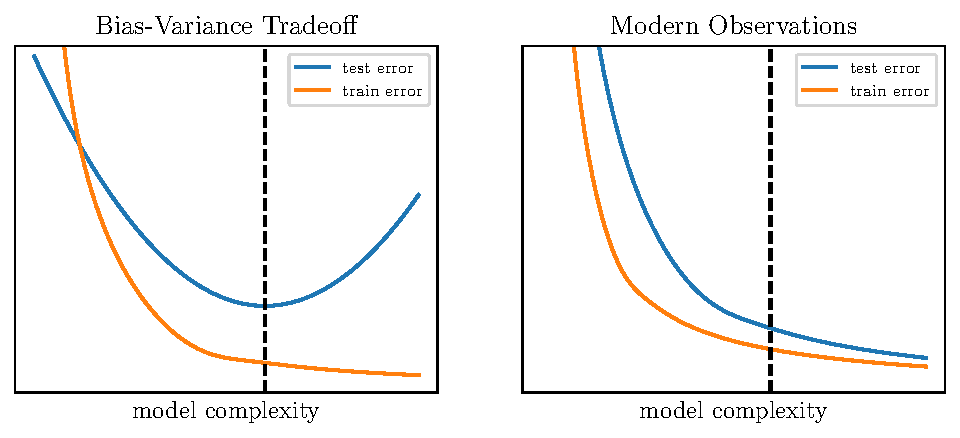
\includegraphics[width=0.8\textwidth, height=0.2\textheight]{old_new.pdf}
		\caption{Common wisdom and many empirical observations suggest that the training error decreases with the complexity of the hypothesis class. The test error decreases as well, only to increase again after a certain threshold as shown in the figure on the left. Here, the threshold usually corresponds to the point where the number of learnable parameters equals the size of the dataset. However, modern observations suggest that deep neural networks can have many parameters and still generalize well as shown in the figure on the right.}
\end{figure}
Recently, there has been a lot of research to understand the phenomenon of
overparameterization. While we will not delve into the details of this research,
we look at a one specific example. 
\begin{boxedexample}
	\label{ex:generalization}
	Consider as a hypothesis class the space of 2-layer neural networks with ReLU
	activation functions. Assume that the learnable weights
	corresponding to the first layer do not deviate much in the 2-norm from
	their initial values. Further, assume that the weights of the second layer
	remain bounded in the 2-norm throughout the training. Formally, this class can be written as
	$$
		\mathfrak{H} := \{h(x) = V \cdot [U\cdot x]_+: U, V \in W\},
		$$
		where
		\begin{align*}
		W :=& \{(U,V) \quad U \in \mathbb{R}^{n \times n_{\text{hu}}}, V \in \mathbb{R}^{n_\text{hu} \times n_{\text{class}}} \quad \text{and}\\
		& \quad \|u_i-u_i^0\|_2 \leq \beta, \|v_i\|_2 \leq \alpha \quad \text{for all units}\}, 
		\end{align*}
		and $n_\text{hu}$ is the number of hidden units, $n_{\text{class}}$ is the
		number of classes, $[.]_+$ denotes the ReLU activation function, $u_i$,
		$v_i$ denote the $i$-th column of $U$ and $V$, respectively, $u_i^0$, $v_i^0$ are the $i$-th column of the
		initial weight matrix $U$, and $V$, respectively, and $\beta$ and $\alpha$ are
		constants.		

		Train such a neural network on the publicly available CIFAR-10 dataset.
		Study empirically both the training error and the test error as a
		function of the number of hidden units. What do you observe? Experiment
		with $n_{\text{hu}}$ ranging from 8 to 30000. 

		Now, empirically study the quantities $\|U\|_2$, $\|V\|_2$, and
		$\|U-U^0\|_2$ as a function of the number of hidden units. What do you observe?
\end{boxedexample}

In \cite{Neyshabur:arXiv1805} the authors did the empirical study explained in
\Cref{ex:generalization} and observed the following:
\begin{itemize}
	\item Both the training error and test error decrease as a function of
	$n_{\text{hu}}$. This indicates that we are in the overparameterization
	regime.
	\item The quantity $\|U\|_2$ initially decreases as a function of
	$n_{\text{hu}}$ and then increases. The quantities $\|V\|_2$ and
	$\|U-U^0\|_2$ decrease as a function of $n_{\text{hu}}$. 
\end{itemize}
The second observation, and specifically the decrease of $\|U-U^0\|_2$ as a
function of $n_{\text{hu}}$, is particularly interesting. It suggests that the
weights of the neural network do not deviate much from their initial values
during training. It appears here that training the neural network is then more
focused on optimizing the weights of the second layer. When interpreting the
hidden units as features, this result suggests that when one has many features,
one has consequently many relevant features that are useful for the task at
hand. Hence, there is no need to learn new features. 

In a next step, the authors bounded the Rademacher complexity of the specific
hypothesis class in \Cref{ex:generalization} by the quantities $\|U-U^0\|_2$ and
$\|V\|_2$. In particular, they showed that
$$
\text{Rad}(l \circ \mathfrak{H} \circ D) \leq \frac{C}{\sqrt{m}} \max_i \|x_i\|_2 \ \alpha \ (\beta+ \|U^0\|_2)
$$

This suggests that the Rademacher complexity of the
hypothesis class decreases as a function of $n_{\text{hu}}$, which is in
line with the empirical observations.

\section*{Wait! What is what?}
Here is a list of questions that help you check your understanding of key
concepts inside this chapter.

\begin{enumerate}
    \item What is the ultimate goal of a supervised learning problem? 
    \item  Where does the randomness in probably-approximately-correct (PAC) learning come from?
    \item What is the realizability assumption in PAC learning?
    \item What is the empirical risk minimization principle?
    \item How do we judge whether a certain type of a complexity measure of a hypothesis class is good?
    \item What is the bias-variance tradeoff? How does it relate to the complexity of the hypothesis class?
    \item What are the limitations of the VC-dimension as a complexity measure of a hypothesis class?
    \item What is the overparameterization regime?
\end{enumerate}

